\documentclass[../TDO1-O2.tex]{subfiles}%

\begin{document}
\section[s]"2"{Détecteur de pluie sur un pare-brise}

\enonce{%
	\noindent
	\begin{minipage}[c]{.68\linewidth}
		On modélise un pare-brise par une lame de verre à faces parallèles, d'épaisseur
		$e = \SI{5.00}{mm}$, d'indice $n_v = \num{1.5}$. Un fin pinceau lumineux issu d'un
		émetteur situé en E arrive de l'intérieur du verre sur le dioptre verre
		$\rightarrow$ air en I avec un angle d'incidence $i = \ang{60.;;}$.
	\end{minipage}
	\hfill
	\noindent
	\begin{minipage}[c]{.30\linewidth}
		\begin{center}
			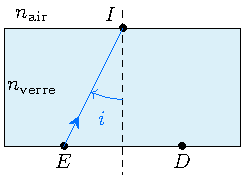
\includegraphics[width=\linewidth]{pluie_plain.pdf}
			\label{fig:pluie_plain}
		\end{center}
	\end{minipage}
}%

\QR{%
	Montrer que le flux lumineux revient intégralement sur le détecteur
	situé en D et déterminer la distance ED.
}{%
	Pour savoir si le pinceau lumineux revient intégralement, il faut
	savoir s'il y a réflexion totale à l'interface verre$\rightarrow$air.
	Pour cela, on utilise la formule de l'angle limite de réfraction
	\begin{equation*}
		i_{\rm lim} = \arcsin \left( \frac{n_2}{n_1} \right)
	\end{equation*}
	Ici, on a
	\[\boxed{i_{\rm lim, v\rightarrow a} =
			\arcsin \left( \frac{n_{\rm air}}{n_{\rm verre}} \right)}
		\quad\text{avec}\quad
		\left\{
		\begin{array}{rcl}
			n_{\rm air}   & = & \num{1.00} \\
			n_{\rm verre} & = & \num{1.5}
		\end{array}
		\right.
	\]
	L'application numérique donne
	\begin{empheq}[box=\fbox]{equation*}
		i_{\rm lim, v\rightarrow a} = \ang{41.8;;}
	\end{empheq}
	Comme $i = \ang{60.;;}$, $i > i_{\rm lim v\rightarrow a}$, et on a
	donc réflexion totale~: aucun rayon ne sera réfracté.\bigbreak
	Avec la figure ci-après, on a $\tan(i) = \frac{\\rm  ED}{2e}$, soit
	\[\boxed{{\rm ED} = 2e\tan(i)}
		\quad\text{avec}\quad
		\left\{
		\begin{array}{rcl}
			e & = & \SI{5.00}{mm} \\
			i & = & \ang{60.;;}
		\end{array}
		\right.\]
	L'application numérique donne
	\begin{empheq}[box=\fbox]{equation*}
		ED = \SI{1.7}{cm}
	\end{empheq}
}%

\QR{%
	Lorsqu'il pleut, une lame d'eau d'indice $n_e = \num{1.33}$ et
	d'épaisseur $e' = \SI{1.00}{mm}$ se dépose sur un pare-brise. Représenter
	le rayon lumineux dans ce cas. À quelle distance du détecteur
	arrive-t-il~?
}{%
	Dans le cas où une fine couche d'eau recouvre le verre, on doit
	calculer le nouvel angle limite de réfraction pour l'interface
	verre$\rightarrow$eau. Comme précédemment, on utilise la formule et on
	trouve
	\begin{empheq}[box=\fbox]{equation}
		i_{\rm lim, v\rightarrow e} = \ang{62.5;;}
	\end{empheq}
	Cette fois, l'angle d'incidence $i < i_{\rm lim, v\rightarrow e}$. On
	va donc avoir réfraction. On détermine l'angle de réfraction $i_2$
	avec la loi de \textsc{Snell-Descartes} pour la réfraction~:
	$n_2\sin(i_2) = n_1\sin(i_1)$. Dans notre cas, $n_2 = n_{\rm eau}$,
	$n_1 = n_{\rm verre}$ et $i_1 = i$~; on aura donc
	\[
		\boxed{i_2 = \arcsin \left(
			\frac{n_{\rm verre}\sin(i)}{n_{\rm eau}}
			\right)}
		\quad\text{avec}\quad
		\left\{
		\begin{array}{rcl}
			n_{\rm verre} & = & \num{1.5}   \\
			i             & = & \ang{60.;;} \\
			n_{\rm eau}   & = & \num{1.33}
		\end{array}
		\right.
	\]
	D'où
	\begin{empheq}[box=\fbox]{equation*}
		i_2 = \ang{77.6;;}
	\end{empheq}
	Ce rayon réfracté (en vert sur la figure) va ensuite rencontrer le
	dioptre eau$\rightarrow$air en $J$, pour lequel l'angle limite de
	réfraction est
	\begin{empheq}[box=\fbox]{equation*}
		i_{\rm lim, e\rightarrow a} = \ang{48.8;;}
	\end{empheq}
	Comme $i_2 > i_{\rm lim, e\rightarrow a}$, on a une nouvelle réflexion
	totale avec $r'=-i_2$, ramenant le pinceau vers le dioptre
	eau$\rightarrow$verre en un point K. Dans cette situation comme la
	valeur absolue de $r'$ est la même que celle de $i_2$, le principe
	du retour inverse de la lumière nous permet de déterminer directement
	que l'angle de réfraction de l'eau vers le verre $i_3$ a la même valeur
	absolue que l'angle d'incidence du verre vers l'eau $i_1$.\bigbreak

	Avec le schéma ci-après, on peut déterminer que $\rm DL = IK$
	(l'abscisse supplémentaire du trajet dans l'eau) et utiliser la
	trigonométrie pour trouver
	\[
		\boxed{{\rm IK} = 2e'\tan(i_2)}
		\quad\text{avec}\quad
		\left\{
		\begin{array}{rcl}
			e'  & = & \SI{1.00}{mm} \\
			i_2 & = & \ang{77.6;;}
		\end{array}
		\right.\]
	soit
	\[
		\boxed{{\rm DL} = \SI{0.9}{cm}}
	\]
	Ainsi, le rayon ne tombe plus sur le détecteur mais à côté~; un système
	de commande relié au détecteur peut alors déclencher les essuie-glaces.
	\begin{center}
		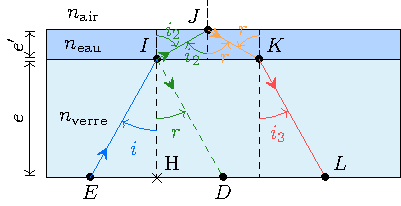
\includegraphics[width=.7\linewidth]{pluie.pdf}
		\label{fig:pluie}
	\end{center}
}%

\end{document}
